\documentclass[paper]{aiaaNew}

\usepackage{esevct}
\usepackage{amssymb}
\usepackage{bm}
\usepackage{amsthm}% http://ctan.org/pkg/amsthm
\usepackage{amsmath}
\usepackage[linewidth=1pt]{mdframed}
\usepackage{graphicx}
\usepackage{algorithm}


% \newenvironment{proof}
% {}{}


%\documentstyle[10pt,draft,fancyheadings]{AIAAtran}
%\documentstyle[9pt,twocolumn,technote,twoside]{AIAAtran}


\SubmitName{Lysandrou}

% for conference paper:

\PaperNumber{xxx}

\CoverFigure{}

\Conference{{\bfseries AIAA Guidance, Navigation and \\ Control 
Conference} \\
            August 10--12,~1998 / Boston, MA}

% for a journal simulation cover page:

\JournalName{Journal of Guidance, Navigation and Control}
\JournalIssue{Volume~xx, Number~xx, Jan.--Feb., 2001, Pages xx--xx}

% journal article simulation:

\ArticleIssue{Vol.~24, No.~1, Jan.--Feb., 2001}% first page
\ArticleHeader{Schaub Et Al: New Penalty Functions}% subsequent pages

% journal note simulation:

\NoteHeader{J.Guidance, Vol.~20, No.~13: Engineering Notes}

% set copyright and other notices to appear
% as a footnote at the bottom of the first page:

%\PaperNotice{\CopyrightB{1998}{Hanspeter Schaub}}

\JournalNotice{Presented as Paper~06--3792 at the AIAA
               Guidance, Navigation and Control Conference, San 
Diego,~CA,               July~29--31,~1996.
               \CopyrightB{1996}{the authors}}
% load the title, author, and abstract for use with the \maketitle command

\title{Attitude Dynamics and Control of a Nano-Satellite Orbiting Mars}
\author{Padraig S. Lysandrou
  \thanks{PhD Student, Aerospace Engineering Department.  Student Member of AIAA.}
  \\
  \emph{\normalsize The University of Colorado Boulder, Boulder, CO 80301}
}

\abstract{
Abstract should be around 200--300 words.  Explain briefly what the problem is, how does the presented work contribute.  Summarize the paper results
}


\begin{document}


\maketitle
\clearpage
\section{Introduction}



 \subsection{Testing of a Subsection}
 \subsubsection{Testing of a Subsection}

\section{Problem Statement}
Let us begin with defining the orbit with the following figure


\begin{figure}[!htbp] 
  \centering
  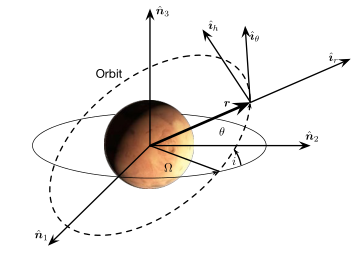
\includegraphics[width=0.5\textwidth]{\Figures/framedef.PNG}
  \caption{Illustration of the Inertial, Hill, and perifocal geometrical constructions.}
  \label{fig:succ}
 \end{figure}



\section*{Task 1: Orbit Simulation}
Our Hill frame is defined by the basis: $\{\bm{\hat{i}}_r, \bm{\hat{i}}_\theta, \bm{\hat{i}}_h \}$ with the inertial defined as $\{\bm{\hat{n}}_1, \bm{\hat{n}}_2, \bm{\hat{n}}_3 \}$. Given the inertial and Hill frame definitions, we know that the position vector of the LMO satellite is $r\bm{\hat{i}}_r$. Additionally we know that since it is a circular orbit, it has a time invariant angular rate ${\bm{\omega}}_{H/N} = \dot{\theta}\mathbf{\hat{i}}_h$. Calculating the vectorial inertial derivative:

\begin{align}
	\dot{\bm{r}} = \frac{^N d}{dt}\bm{r} &= \frac{^H d}{dt}\bm{r} + \bm{\omega}_{H/N} \times \bm{r} \\
	&= \dot{\theta}\bm{\hat{i}}_h \times r\bm{\hat{i}}_r \\
	&= r\dot{\theta} \bm{\hat{i}}_\theta
\end{align}

Additionally, we can use this information to find the inertial position and velocity vectors by performing transformations using the perifocal frame information. We know that the perifocal frame can be defined by an Euler 3-1-3 rotation.  









\section{Numerical Simulations}

\section{Conclusion}

\section*{Acknowledgment}

\bibliographystyle{aiaa}   % Number the references.
\bibliography{references}   % Use references.bib to resolve the labels.


\end{document}

